\documentclass[11pt, ngerman, fleqn, DIV=15, headinclude, BCOR=2cm]{scrreprt}

\usepackage{../../header}

\usepackage{placeins}
\usepackage[maxfloats=50]{morefloats}
\usepackage{subcaption}

\usepackage{csquotes}

\usepackage{tikz}
\usetikzlibrary{chains}
\usetikzlibrary{shapes.geometric}

\tikzset{device/.style={
                rectangle,
                minimum size=6mm,
                draw=black
            },
            monitor/.style={
                rectangle,
                rounded corners=2mm,
                minimum size=6mm,
                draw=black
            },
        }

\usepackage{pgfplots}
\pgfplotsset{
    compat=1.9,
    width=0.8\linewidth,
    xticklabel style={/pgf/number format/use comma},
    yticklabel style={/pgf/number format/use comma},
}
\usepgfplotslibrary{polar}

\usepgfplotslibrary{external}
\tikzexternalize[mode=list and make]
\tikzsetexternalprefix{Abbildung-}

\DeclareSIUnit{\skt}{SKT}

\usepackage{booktabs}

\hypersetup{
    pdftitle=
}

\newcommand{\plotwidth}{0.8\linewidth}

\subject{Praktikumsprotokoll}
\title{$\gamma$-Spektroskopie mit Szintillations- und Halbleiterdetektoren}
\subtitle{Versuch P521 -- Universität Bonn}
\author{
	Frederike Schrödel \\
	\small{\href{mailto:fschroedel@gmx.de}{fschroedel@gmx.de}}
	\and
	Simon Schlepphorst \\
	\small{\href{mailto:s2@uni-bonn.de}{s2@uni-bonn.de}}
}

\date{2015-11-09 bis 11-12}

\publishers{Tutor: Philipp Hoffmeister
}

\begin{document}

\maketitle

\begin{abstract}
    In diesen Versuch geht es darum, die Eigenschaften von einem
    Szintillationsdetektor und einem Ge-Halbleiterdetektor bei der
    $\gamma$-Spektroskopie zu vergleichen.
    Dabei sind die Energieauflösung und die Nachweiswahrscheinlichkeit die
    zu untersuchenden Eigenschaften.
\end{abstract}


\tableofcontents

\chapter{Theorie}

\section{Wechselwirkung von $\gamma$-Strahlung mit Materie}

Die $\gamma$-Strahlung entsteht wenn nach einem vorhergegangen Zerfall der
Tochterkern nicht in seinen Grundzustand, sondern in einen angeregten Zustand
zerfällt.
Dieser angeregte Zustand zerfällt nach einiger Zeit durch Abstrahlung des
$\gamma$-Quants in den Grundzustand. Diese Photonen sind sehr energiereich,
weshalb sie genug Energie haben, um auf verschiedene Weisen mit der Materie zu
Wechselwirken.
Die Art diese Wechselwirkung hängt von der Ordnungszahl der bestrahlten Atome
und der Energie der $\gamma$-Strahlung ab.

\subsection{Photoeffekt}

Der Photoeffekt beschreibt den Vorgang, bei welchem ein Photon ein Elektron aus
dem Atom auslöst.
Hierbei gibt das Photon seine komplette Energie ab.
Die kinetische Energie des ausgelösten Elektrons hängt nur über die
Bindungsenergie ($E_\text{Bind.}$) mit dem der Energie des Photons ($h\nu$),
also dessen Frequenz ($\nu$) zusammen.
Dieser Prozess kann nur in der Nähe eines Atomkerns stattfinden weil dieser
den Rückstoß aufnimmt.
So bleibt bei diesen Vorgang Energie und Impuls erhalten. 
\[ 
    E = h\nu - E_\text{Bind.}
\]
Wenn man sich den Wirkungsquerschnitt $\sigma$ für diesen Prozess anschaut,
dann stellt man eine große Abhängigkeit von der Ordnungszahl $Z$ fest.
\[
    \sigma \propto Z^5 E_\gamma^{\frac 72}
\]
Deshalb tritt dieser Effekt besonders häufig bei Elementen mit hoher Ordnungszahl
auf.

\subsection{Paarerzeugung}

Ein weiterer Effekt, der bei Energien $E_\gamma \ge 2m_\text ec^2$ auftreten
kann, ist die Elektron-Positron-Paarbildung.
Dieser Effekt ist allerdings erst weit oberhalb dieser Schwelle relevant.
Für den Wirkungsquerschnitt gilt $\sigma \propto Z^2$.

\subsection{Comptonstreuung}

Wenn Photonen an einem Elektron streuen, dann spricht man vom Comptoneffekt. 
Hierbei gibt das Photon einen Teil seiner Energie an das Elektron ab und ändert dabei
seine Frequenz.
Die abgegebene Energie hängt dabei vom Streuwinkel ab.
Für die Restenergie des Photons gilt:
\[
    E_\nu'(\phi) = \frac{E_\nu}{1+\frac{E_\nu}{m_\text ec^2}(1+\cos(\phi))}
\]
Die größte Energieänderung erhält man also bei einem Winkel von
$\phi=\SI{180}{\degree}$.
Diese Energieänderung berechnet sich durch:
\[
    \delta\lambda = \frac{h}{m_\text ec}(1-\cos(\phi))
\]
Der Wirkungsquerschnitt entspricht $\sigma_\text C \propto \frac{Z}{E_\gamma}$.

\subsection{Keine Wechselwirkung}

Ein nicht unerheblicher Teil der $\gamma$-Strahlung kann auch Wechselwirkung
Materie durchdringen.

\section{Szintillationsdetektor}

Mit einem Szintillationsdetektor lassen sich Intensität und Energie von
ionisierender Strahlung messen.
Er besteht aus einem Szintillator und einem Photomultiplier.
Der Szintillator ist ein dotierter Einkristall, der von energiereicher
Strahlung zum Fluoreszieren angeregt werden kann und hinreichend
durchlässig für das von ihm emittierte Licht ist.

Innerhalb des vor Lichteinfall geschützten Szintillators entstehen durch
ionisierende Strahlung Lichtblitze. 
Wie viele dieser Blitze auftreten ist von der Energie der Strahlung abhängig.
Aufgrund des Photoeffektes werden an der Photokathode des Photomultipliers
Elektronen ausgelöst.
% FIXME Was soll der folgende Satz?
Durch den Aufbau weitern des Photomultiplieres kommt es zu einem Lawineneffekt,
welcher die Elektronen vervielfacht und somit eine Detektion erleichtert.
Die Amplitude des so entstanden Strompulses ist somit auch proportional zu der
Energie der Eingangsstrahlung.

Wenn man eine gute Energieauflösung möchte, sollte man allerdings eher einen
Halbleiterdetektor nutzen.

% TODO Und warum sollte man das?

\section{Halbleiterdetektor}

Die Basis des Halbleiterdetektors bildet die Verarmungszone, die zwischen einem
$p$- und einem $n$-dotieren Halbleiter entsteht.

Betrachtet man das Bändermodel vom Halbleitern, so kann man sich die Dotierung
des Halbleiters als weiteres dünnes Band knapp unter dem Leitungsband
($n$-dotiert) oder knapp über dem Valenzband ($p$-dotiert) vorstellen.
Dabei erhält man die Dotierung eines Kristalls indem man fremde Atome in den
Kristall einbindet.
Wenn man eine positive Dotierung möchte, so fügt man in den Kristall Atome mit
einer niedrigeren Anzahl Valenzelektronen ein, für die negative Dotierung nutzt
man Atome mit höherer Valenzelektronenanzahl.

Fügt man diese beiden Bereiche aneinander, so entsteht dazwischen eine Bereich,
indem die überschüssigen Elektronen aus dem $n$-dotierten Teil in den
$p$-dotierten Bereich übergehen.
Hierdurch bildet sich durch die zurückbleibenden Ionenrümpfe ein elektrisches Feld aus, welches
der weitern Verbreiterung der Verarmungszone entgegen wirkt.
Es entspricht somit einer Diode.
Wenn man diese nun in Sperrrichtung betreibt, kann man die Verarmungszone weiter
verbreitern.
Das ist erwünscht, da nur in diesen Bereich des Detektors Ereignisse
gemessen werden können.

\subsection{Multi-Channel-Analyzer}

Um ein nach Amplituden sortiertes Spektrum zu erhalten, nutzen wir ein MCA.
Dies ist ein Bauteil, welches einkommende Signale nach Amplitude sortiert und
dann den Kanal, welcher der Impulshöhe entspricht, hoch setzt. So erhalten wir ein
Histogramm.

%TODO Bild Spektrum
%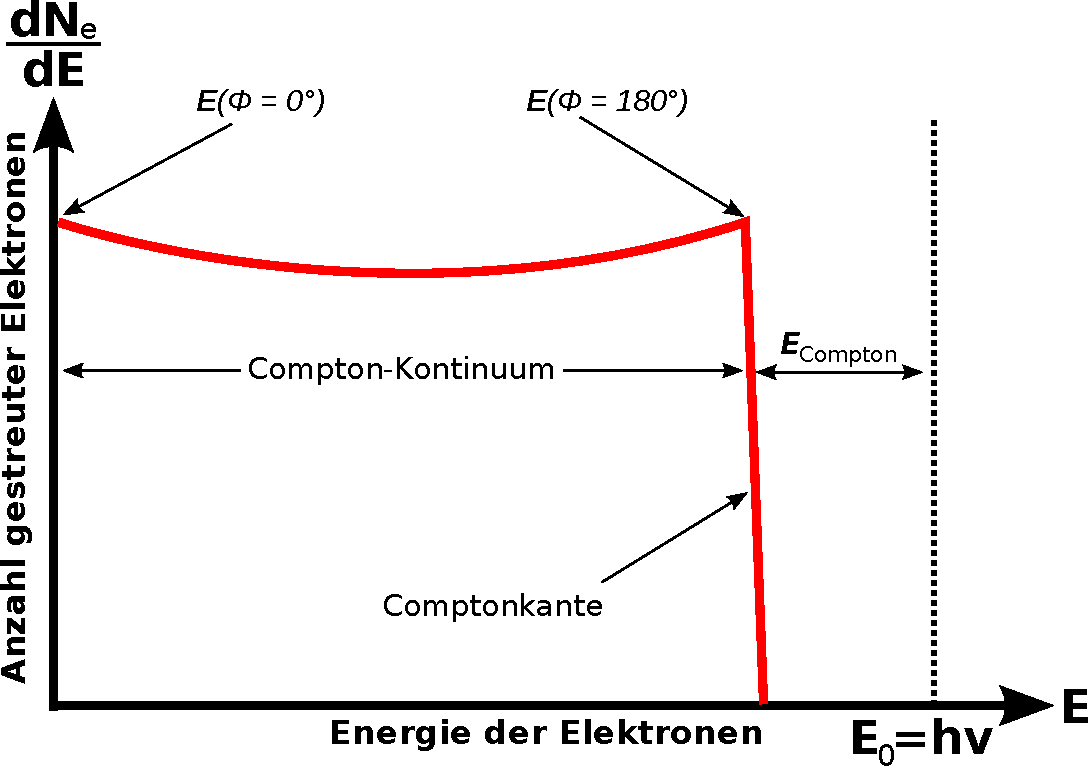
\includegraphics[width=0.5\linewidth]{../graphics/Compton-spektrum.pdf}
%\parencite{comptoneffekt}

%In dem entstehenden Spektrum, erkennt man ein Compton-Kontinuum, welches die 
%Comptonstreuung bis zu einem Winkel von \SI{180}{\degree} enthält. Da bei diesem
%Wert der maximale Energieübertrag stattfindet, erhält man eine scharfe Kante, 
%die Compton Kante. Wird nicht nur ein Teil sondern die gesamte Energie
%abgegeben, wie es beim
%Photoeffekt der Fall ist, entsteht der energetisch höher gelegene Ausschlag. Man 
%nennt ihn Photo-Peak.



\chapter{Aufbau und Durchführung}

Der Aufbau dieses Experiments sieht wie folgt aus:

Der jeweilige Detektor ist an einen Signalverstärker angeschlossen, welcher
wiederum an einen Vielkanalanalysator angeschlossen ist.

Für die Durchführung müssen zunächst die Betriebsparameter, wie die
Verstärkung des Signalverstärkers eingestellt werden.
Dazu werden die Proben jeweils einzeln vor die Detektoren gestellt und das
Ausgangssignal des Signalverstärkers am Oszilloskop betrachtet.
Die Verstärkung ist so eingestellt, dass die für die Energiekalibrierung
wichtige \SI{1408}{\kilo\electronvolt}-Linie des $^{152}\text{Eu}$
innerhalb des Messbereichs liegt.
%TODO Foto vom Aufbau

Nun messen wir mit beiden Detektoren sowohl die drei Proben, $^{60}\text{Co}$,
$^{137}\text{Cs}$ und $^{152}\text{Eu}$, als auch den Untergrund. Jede dieser
Messungen wird über einen Zeitraum von fünf Minuten aufgenommen.

Für die Langzeitmessung mit dem Ge-Detektor wird eine Bleiabschirmung
aufgebaut, mit der über Nacht der Untergrund gemessen wird bevor die Bodenprobe
innerhalb der Abschirmung positioniert wird und erneut über Nacht gemessen wird.

\chapter{Auswertung}

Bevor wir anfangen können die Spektren zu untersuchen, müssen zunächst die
Aufnahmezeiten angepasst werden, da wir die Realzeit auf \SI{600}{\second} gesetzt
haben und diese durch Totzeiten des Detektors von der Aufnahmezeit abweicht.
Nach Anpassung der Zeit müssen wir die
Untergrundmessung von der Messung der Spektren abziehen.
Von den gefilterten Spektren untersuchen wir im folgenden die durch
$\gamma$-Zerfall entstandenen Ausschläge. Abbildung~\ref{fig:energiekalibrierung}
% FIXME Satzende?

\begin{figure}
    \centering
    \includegraphics[width=\plotwidth]{Ge_calib}
    \caption{%
	    $^{152}\text{Eu}$-Spektrum im Ge-Detektor
        %
    }
    \label{fig:energiekalibrierung}
\end{figure}

Da die Spektren mit einem Vielkanalanalysator aufgenommen werden, muss eine
Energiekalibrierung vorgenommen werden. Hierbei wird den Nummern der 8192
Kanäle die Energie zugeordnet der sie entsprechen.
Das lässt sich erreichen indem wir durch Anpassen von Verteilungsfunktionen an die
Ausschläge bekannter $\gamma$-Übergänge deren Schwerpunkt in Kanalnummer
erhalten. An die Daten aus dem NaJ(Ti)-Detektor haben wir Gaußkurven und an die
aus dem Ge-Detektor Lorentzkurven angepasst, da diese näher an den Daten liegen.
Somit wurde den Kanalnummern eine Energie zugeordnet. Abbildung~\ref{fig:Ge-peaks}
% FIXME Satzende?

\begin{tabular}{SSSSSS}
    {Nummer} & {Kanal} & {Breite $\Gamma$} & {Fläche} & {rel.\ Intens.} &
    {$E_\gamma$ / \si{\kilo\electronvolt}} \\
    \midrule
    %< for row in sz_fits_table >%
    << ' & '.join(row) >> \\
    %< endfor >%
\end{tabular}

Für den NaJ(Ti)-Detektor nutzen wir die beiden am besten getrennten Linien des
$^{152}\text{Eu}$: die Linie des $^{137}\text{Cs}$ und die Linien des
$^{60}\text{Co}$.

\begin{tabular}{SSSSSS}
    {Nummer} & {Kanal} & {Breite $\Gamma$} & {Fläche} & {rel.\ Intens.} &
    {$E_\gamma$ / \si{\kilo\electronvolt}} \\
    \midrule
    %< for row in ge_eu_fits_table >%
    << ' & '.join(row) >> \\
    %< endfor >%
    \midrule
    %< for row in ge_cs_fits_table >%
    << ' & '.join(row) >> \\
    %< endfor >%
    \midrule
    %< for row in ge_co_fits_table >%
    << ' & '.join(row) >> \\
    %< endfor >%
\end{tabular}

Da die Energieauflösung des Ge-Detektors deutlich besser ist als die des 
NaJ(Ti)-Detektors lassen sich deutlich mehr Linien des $^{152}\text{Eu}$
erkennen und trennen sodass wir davon sieben verwerten konnten.

\begin{figure}
    \centering
    \includegraphics[width=\plotwidth]{Ge_calib-peaks}
    \caption{%
	    Spitzen des $^{152}\text{Eu}$-Spektrums aus dem Ge-Detektor  mit
	    angepassten Lorentz-Kurven
        %
    }
    \label{fig:Ge-peaks}

\end{figure}

Das Energie-zu-Kanal Verhältnis haben wir grafisch in
Abbildung~\ref{fig:ge_kanal} für den
Ge-Detektor und in Abbildung~\ref{fig:sz_kanal} für den NaJ(Ti)-Detektor aufgetragen.
Die angepassten Geraden haben folgende Werte:

NaJ(Ti)-Detektor
\[
    \text{Energie} =
    \text{Kanalnummer} \cdot \SI{<< sz_slope >>}{\kilo\electronvolt}
    +
    \SI{<< sz_offset >>}{\kilo\electronvolt} \,.
\]
Ge-Detektor
\[
    \text{Energie} =
    \text{Kanalnummer} \cdot \SI{<< ge_slope >>}{\kilo\electronvolt}
    +
    \SI{<< ge_offset >>}{\kilo\electronvolt} \,.
\]

Da wir bereits Lorentz- und Gaußkurven angepasst haben um den Schwerpunkt zu
bestimmen, kennen wir auch die Halbwertsbreiten $\Gamma$.

\begin{align*}
	f_\text{Gauß}\del x &= \frac1{\sigma \sqrt{2\pi}}
	\eup^{-\frac12\del{\frac{x
	- \langle x\rangle}{\sigma}}^2}\\
	\\
	f_\text{Lorentz}\del x &= \frac1\pi \frac\sigma{\del{x - \langle x
	\rangle}^2 + \sigma^2}\\
	\\
	\text{mit } \Gamma &= 2 \sigma
\end{align*}

%TODO kommentar zur detektor abhängigkeit.
Diese zeigen auch wieder, um wie viel besser die Energieauflösung des
Ge-Detektors ist.

Aus den Halbwertsbreiten der Linien, die mit dem Ge-Detektor aufgenommen
wurden,
lässt sich die intrinsische Halbwertsbreite $\Delta E_d$ bestimmen.
\[
	\Delta E_d(E_\gamma)=\text{Const}\cdot\sqrt{E_\gamma}
\]
Dieser Zusammenhang wurde in Abbildung~\ref{fig:halbwertsbreite} untersucht und die Konstante
ermittelt.
Mit dem Wert, den wir für die intrinsische Halbwertsbreite gefunden haben, lässt
sich wie folgt der elektronische Anteil der Halbwertsbreite bestimmen.
\[
	\Delta E(E_\gamma)=\sqrt{\Delta E_d(E_\gamma))^2+(\Delta E_e)^2}
\]
Wir erhalten:
\[
    \text{Const} = \num{<< ge_const >>}\,\sqrt{\si{\kilo\electronvolt}}
    ,\qquad
    \Delta E_\mathrm e = \SI{<< ge_electronic_width >>}{\kilo\electronvolt}
\]

Nun soll das Verhältnis der Ereignisse im Photopeak gegenüber allen Ereignissen
im Detektor gebildet werden (Peak-to-Total-Verhältnis). Dies wird mit dem
Einzelpeak von $^{137}\text{Cs}$ und dem Summe aus dem Doppelpeak von
$^{60}\text{Co}$ durchgeführt:

NaJ(Ti)-Detektor
\[
    \text{Peak-to-Total (Cs, \SI{662}{\kilo\electronvolt})} = \num{<< sz_cs_ptt >>}
\]
\[
    \text{Peak-to-Total (Co, \SI{1250}{\kilo\electronvolt})} = \num{<< sz_co_ptt >>}
\]
Ge-Detektor
\[
    \text{Peak-to-Total (Cs, \SI{662}{\kilo\electronvolt})} = \num{<< ge_cs_ptt >>}
\]
\[
    \text{Peak-to-Total (Co, \SI{1250}{\kilo\electronvolt})} = \num{<< ge_co_ptt >>}
\]


Die absolute Peakeffizienz wird aus dem Verhältnis der Ereignisse im Photopeak
und aller ausgestrahlten $\gamma$-Quanten der Probe gebildet. Dazu benutzen wir
die bekannten Werte der $^{137}\text{Cs}$ Probe (\SI{0.925}{\mega\becquerel},
April 1985). Daraus erhalten wir eine aktuelle Aktivität von:
\[
	A\del{^{137}\text{Cs}} = \SI{<< cs_activity >>}{\becquerel}
\]
Bei einem Abstand von etwa \SI{25}{\centi\metre} zwischen Detektor und Probe
erhalten wir:

NaJ(Ti)-Detektor
\[
    \text{Absolute Peakeffizienz (Cs)} = \num{<< ge_cs_abs >>}
\]
Ge-Detektor
\[
    \text{Absolute Peakeffizienz (Cs)} = \num{<< sz_cs_abs >>}
\]


Um die relative Effizienz des Ge-Detektors zu bestimmen ermitteln wir die
relative Intensität aus der Fläche und der Energie der verschiedenen
$^{152}\text{Eu}$ Linien und normieren diese auf eine relative Intensität der
\SI{1408}{\kilo\electronvolt} Linie von 1000.
In Abbildung~\ref{fig:effizienz} ist die relative Effizienz aufgetragen, indem
wir die ermittelten relativen Intensitäten durch die erwarteten relativen
Intensitäten der $\gamma$-Linien geteilt haben.

\begin{tabular}{SSSS}
    {Energie / \si{\kilo\electronvolt}} & {rel.\ Intens. erw.} & {rel.\ Intens.
mess.} & {Effizienz} \\
    \midrule
    %< for row in ge_efficiency_table >%
    << ' & '.join(row) >> \\
    %< endfor >%
\end{tabular}

%\begin{figure}
%    \centering
%    \includegraphics[width=\plotwidth]{Ge_calib}
%    \caption{%
%        %
%    }
%    \label{fig:energiekalibrierung}
%\end{figure}

%\begin{figure}
%    \centering
%    \includegraphics[width=\plotwidth]{Ge_calib-peaks}
%    \caption{%
%        %
%    }
%    \label{fig:Ge-peaks}
%\end{figure}


%Germanium
%\[
%    \text{Energie} =
%    \text{Kanalnummer} \cdot \SI{<< ge_slope >>}{\kilo\electronvolt}
%    +
%    \SI{<< ge_offset >>}{\kilo\electronvolt} \,.
%\]
%\[
%    \text{Peak-to-Total(Cs)} = \num{<< ge_cs_ptt >>}
%\]
%\[
%    \text{Peak-to-Total(Co)} = \num{<< ge_co_ptt >>}
%\]
%\[
%    \text{Absolute Peakeffizienz (Cs)} = \num{<< ge_cs_abs >>}
%\]

\begin{figure}
    \centering
    \includegraphics[width=\plotwidth]{ge_channels}
    \caption{%
	    Energiekalibrierung des Ge-Detektors
        %
    }
    \label{fig:ge_kanal}
\end{figure}


%Szintillationszähler
%\[
%    \text{Energie} =
%    \text{Kanalnummer} \cdot \SI{<< sz_slope >>}{\kilo\electronvolt}
%    +
%    \SI{<< sz_offset >>}{\kilo\electronvolt} \,.
%\]
%\[
%    \text{Peak-to-Total(Cs)} = \num{<< sz_cs_ptt >>}
%\]
%\[
%    \text{Peak-to-Total(Co)} = \num{<< sz_co_ptt >>}
%\]
%\[
%    \text{Absolute Peakeffizienz (Cs)} = \num{<< sz_cs_abs >>}
%\]

\begin{figure}
    \centering
    \includegraphics[width=\plotwidth]{Sz-CO-peaks}
    \caption{%
	    Spitzen des $^{60}\text{Co}$-Spektrums aus dem NaJ(Ti)-Detektor
	    mit angepassten Gauß-Kurven
        %
    }
    \label{fig:}
\end{figure}

\begin{figure}
    \centering
    \includegraphics[width=\plotwidth]{Sz-CS-peaks}
    \caption{%
	    Spitzen des $^{137}\text{Cs}$-Spektrums aus dem NaJ(Ti)-Detektor
	    mit angepassten Gauß-Kurven
        %
    }
    \label{fig:}
\end{figure}

\begin{figure}
    \centering
    \includegraphics[width=\plotwidth]{Sz-EU-peaks}
    \caption{%
	    Spitzen des $^{152}\text{Eu}$-Spektrums aus dem NaJ(Ti)-Detektor
	    mit angepassten Gauß-Kurven
        %
    }
    \label{fig:}
\end{figure}

\begin{figure}
    \centering
    \includegraphics[width=\plotwidth]{sz_channels}
    \caption{%
	    Energiekalibrierung des NaJ(Ti)-Detektors
        %
    }
    \label{fig:sz_kanal}
\end{figure}

%\[
%    \text{Const} = \num{<< ge_const >>}\,\sqrt{\si{\kilo\electronvolt}}
%    ,\qquad
%    \Delta E_\mathrm e = \SI{<< ge_electronic_width >>}{\kilo\electronvolt}
%\]

\begin{figure}
    \centering
    \includegraphics[width=\plotwidth]{halbwertsbreite_ge}
    \caption{%
	    Halbwertsbreite abhängig von der Energie im Ge-Detektor
        %
    }
    \label{fig:halbwertsbreite}
\end{figure}


\begin{figure}
    \centering
    \includegraphics[width=\plotwidth]{ge_efficiency}
    \caption{%
	    Energieabhängige Effizenz des Ge-Detektors.
        %
            Fit mit $a \cdot (E/\si{\kilo\electronvolt})^b + c$ mit
            $a = \num{<< ge_effizienz_a >>}$,
            $b = \num{<< ge_effizienz_b >>}$ und
            $c = \num{<< ge_effizienz_c >>}$.
    }
    \label{fig:effizienz}
\end{figure}

\clearpage

\begin{figure}
    \centering
    \includegraphics[width=\plotwidth]{element_match}
    \caption{%
	    Spektren der Bodenprobe und dazu passender Isotope
        %
    }
    \label{fig:element_match}
\end{figure}

Nachdem nun die Energiekalibrierung vorgenommen und die relative
Effizienz bestimmt wurde, können wir die daraus gewonnenen Informationen nutzen
um den Linien aus der Langzeitmessung der Bodenprobe die Zerfallsisotope
zuzuordnen.
Hierfür haben wir die Informationen über die Energie, sowie die relativen
Intensitäten der $\gamma$-Zerfälle aus einer Datenbank
\parencite{IAEA-gamma-ray-database} entnommen.
Aus dieser Datenbank haben wir Spektren generiert und diese mit unserem gemessen
Spektrum verglichen.
% FIXME Und wie wurden die Spektren generiert? Es wurden die Energien und
% Wirkungsquerschnitte genommen. Die Höhe der Linie wurde als proportional zum
% Wirkungsquerschnitt angenommen. Eine feste Breite, die zu den restlichen
% Linien des Detektors passte, wurde ausgesucht. Mit diesen Parametern
% (Mittelwert, Höhe und Breite) wurde für jede Linie eine Lorentzkurve
% generiert und auf das bisherige Spektrum für dieses Isotop addiert. Am Ende
% gab es so ein Spektrum für jedes Element mit unterschiedlichen Höhen für die
% verschiedenen Zerfallskanäle. Die Spektren wurden dann noch am Stück so
% normiert, dass sie gut zur Messung passen und vergleichbar sind.
Ein Kriterium ist, wie sehr unsere Daten die generierten Spektren
ausfüllen. Wenn alle Linien eines Isotops sowohl in der Lage als auch den
Höhenverhältnissen
mit den entsprechenden Linien des gemessenen Spektrums überein stimmen, so haben
wir dieses Isotop in die engere Auswahl genommen. Wenn nur ein Teil der Linien
übereinstimmt, aber andere Linie nicht in dem gemessen Spektrum vorkommen, so
haben wir dieses Isotop verworfen.
Als nächstes haben wir aus allen möglichen Isotopen ein Spektrum erstellt, um
festzustellen, ob das resultierende Spektrum sich so erklären lässt.
Das Resultat ist in Abbildung~\ref{fig:element_match} zu sehen.
Dabei lassen sich die meisten Isotope natürlichen Zerfallsreihen zuordnen.

\begin{align*}
    \text{Thorium-Reihe:} & ^{212}\text{Pb} \quad \leadsto ^{212}\text{Bi}
    \leadsto ^{208}\text{Tl} \\
    \text{Radon-Reihe:} & ^{214}\text{Pb} \leadsto  ^{214}\text{Bi}
\end{align*}

$^{68}\text{Ga}$ und $^{64}\text{Cu}$ kommen nicht natürlich vor, werden aber
in der Medizin eingesetzt.


\section{Bodenprobe}


\begin{figure}
	\centering
	\includegraphics[width=\plotwidth]{plot_spektren_langzeit}
	\caption{%
		Vergleich von Proben- und Untergrundspektrum
	}
	\label{fig:langzeit_probe_untergrund}
\end{figure}


\begin{figure}
	\centering
	\includegraphics[width=\plotwidth]{plot_peaks_langzeit}
	\caption{%
		Peaks im Probenspektrum
	}
	\label{fig:langzeit_probe_peaks}
\end{figure}



\begin{figure}[h]
	\centering
	\begin{tabular}{SSSS}
		{E / \si{\kilo\electronvolt}} &
		{FWHM / \si{\kilo\electronvolt}} &
            {Intensität / \num{e4}} &
            {Offset / \num{e5}}\\
		\midrule
		%< for row in langzeit_calibration_table: ->%
		<< ' & '.join(row) >> \\
		%< endfor ->%
	\end{tabular}
	\caption{%
		Anpassungsparameter für die Energiekalibrierung
	}
	\label{tab:energiekalibrierung}
\end{figure}


\chapter{Ergebnis}

In diesen Versuch haben wir gut sehen können, dass die Energie- und Zeitauflösung der
beiden Detektoren sehr unterschiedlich ist. Wir haben auch sehen können, dass
die Energiekalibrierung gut funktioniert. 
Dadurch lassen sich gut die Isotope der Bodenprobe bestimmen. Das nicht
alle Linien zugeordnet werden konnten liegt vermutlich daran, dass die
verwendete Datenbank nicht vollständig ist. Die identifizierten Isotope passen
sehr gut zu dem was man erwarten würde. Besonders die deutliche Linie des
nicht natürlich vorkommenden $^{137}\text{Cs}$-Isotops, die sich auf das Unglück
in Tschernobyl zurückführen lässt, ist immer noch deutlich erkennbar, was bei
einer Halbwertszeit von 30 Jahren auch gut möglich ist.

%%%%%%%%%%%%%%%%%%%%%%%%%%%%%%%%%%%%%%%%%%%%%%%%%%%%%%%%%%%%%%%%%%%%%%%%%%%%%%%
%                                   Anhang                                    %
%%%%%%%%%%%%%%%%%%%%%%%%%%%%%%%%%%%%%%%%%%%%%%%%%%%%%%%%%%%%%%%%%%%%%%%%%%%%%%%

\begin{appendix}

\chapter{Anhang}
\section{Bodenprobe}
%TODO

%< for num, first, last, kev in plot_fit_peaks >%
\begin{figure}
    \centering
    \begin{subfigure}{\linewidth}
        \includegraphics[width=.8\linewidth]{plot_fit_peak__<< num >>_langzeit}
        \caption{Rohdaten}
    \end{subfigure}
    \begin{subfigure}{\linewidth}
        \includegraphics[width=.8\linewidth]{element_match_<< num >>_score}
        \caption{Kandidaten nach Übereinstimmung}
    \end{subfigure}
    \begin{subfigure}{\linewidth}
        \includegraphics[width=.8\linewidth]{element_match_<< num >>_contrast}
        \caption{Kandidaten zum Zuordnen}
    \end{subfigure}
    \caption{%
        \SI{<< kev >>}{\kilo\electronvolt}-Linie
        mit Lorentzanpassung
    }
    \label{fig:}
\end{figure}
%< endfor >%

\end{appendix}

\end{document}

% vim: spell spelllang=de tw=79
